\subsection{Session Booking Process Activity}

\begin{figure}[H]
    \centering
    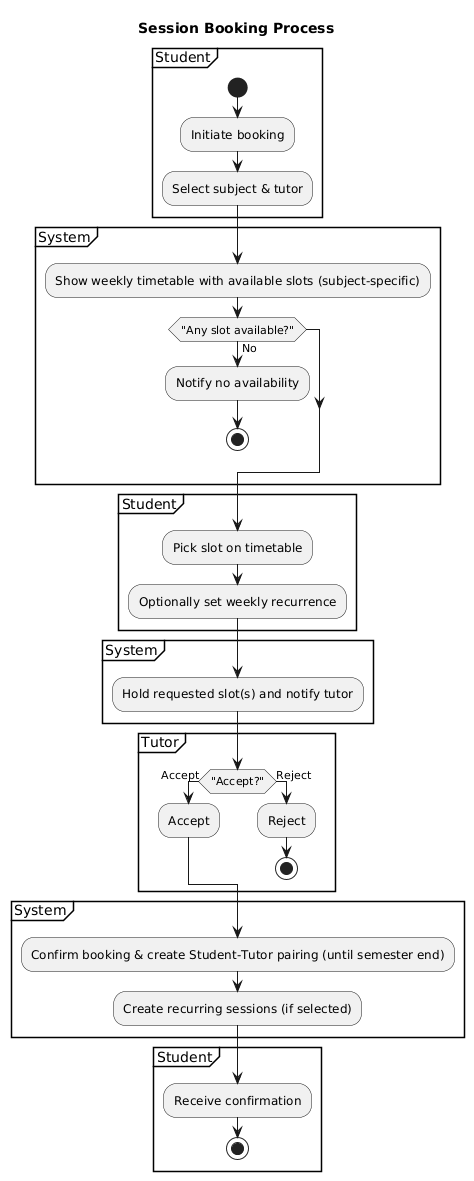
\includegraphics[width=0.45\textwidth]{graphics/chapter4/student/booking.png}
    \caption{Session Booking Process}
    \label{fig:Booking}
\end{figure}

\newpage 

\noindent \textbf{Description}
\begin{enumerate}
  \item \textbf{Student}: Initiates booking; selects subject and a specific tutor.
  \item \textbf{System}: Builds and shows the weekly timetable with subject-specific availability.
  \item \textbf{Decision}: Any suitable slot available?
    \begin{enumerate}
        \item \textbf{Yes:} Continue.
        \item \textbf{No:} System notifies no availability. \emph{Flow ends.}
    \end{enumerate}
  \item \textbf{Student}: Picks a slot on the timetable; optionally sets weekly recurrence.
  \item \textbf{System}: Tentatively holds the requested slot(s) and notifies the tutor.
  \item \textbf{Tutor}: Reviews the request and accepts or rejects.
    \begin{enumerate}
        \item \textbf{Accept:} Continue.
        \item \textbf{Reject:} \textit{Flow ends.}
    \end{enumerate}
  \item \textbf{System}: Confirms booking; then creates a Student–Tutor pairing until the end of semester; schedules recurring sessions (if selected)
  \item \textbf{Student}: Receives confirmation.  \textit{Flow ends.}
\end{enumerate}